\documentclass[a4paper, 12pt]{article}%тип документа



%отступы
\usepackage[left=1cm,right=1cm,top=1cm,bottom=2cm,bindingoffset=0cm]{geometry}

%%% Работа с русским языком
\usepackage{graphicx}
\usepackage{cmap}                           % поиск в PDF
\usepackage{mathtext} 			 	       % русские буквы в формулах
\usepackage[T2A]{fontenc}               % кодировка
\usepackage[utf8]{inputenc}              % кодировка исходного текста
\usepackage[english,russian]{babel} 
\usepackage{float}
\usepackage{sidecap}
\usepackage{graphicx}
\usepackage{wrapfig}
\usepackage{multirow}
\usepackage[export]{adjustbox} % локализация и переносы
\usepackage[unicode, pdftex]{hyperref}
\usepackage{subfig}% http://ctan.org/pkg/subfig
\usepackage{booktabs}

\usepackage{wrapfig}


%Матеша
\usepackage{amsmath,amsfonts,amssymb,amsthm,mathtools} % AMS
\usepackage{icomma} % "Умная" запятая

%\mathtoolsset{showonlyrefs=true} % Показывать номера только у тех формул, на которые есть \eqref{} в тексте.

%% Шрифты
\usepackage{euscript}	 % Шрифт Евклид
\usepackage{mathrsfs} % Красивый матшрифт

%% Свои команды
\DeclareMathOperator{\sgn}{\mathop{sgn}}

%% Перенос знаков в формулах (по Львовскому)
\newcommand*{\hm}[1]{#1\nobreak\discretionary{}
	{\hbox{$\mathsurround=0pt #1$}}{}}
\newcommand{\rref}[1]{(\ref{#1})}
\newenvironment{comment}{}{}
\newcommand{\picref}[1]{рис. \ref{#1}}
\newcommand{\mbf}{\mathbf}
\newcommand{\Equip}[3]{
	
	{\bf #1:} $\Delta = \pm #2$ \si{#3}}
\newcommand{\equip}[1]{
	
	{\bf #1}}

%\usepackage{caption}
%\usepackage{subcaption}


\author{Гаврилин Илья Дмитриевич \\
	Б01-101}
\title{\textbf{Лабораторная работа 4.3.1\\ 
		Изучение дифракции света}}
\begin{document}
	\maketitle
	\section{Аннотация}
	В работе исследовали явления дифракции Френеля и Фраунгофера на одной и двух
	щелях, изучили влияние дифракции на разрешающую способность оптических инструментов; проверили теоретические соотношения для положения максимумов при дифракции Френеля и Фраунгофера.
	\section{Ход работы}
	\subsection{Дифракция Френеля на щели}
	
	\subsubsection{Экспериментальная установка}
	
	Схема установки для наблюдения дифракции Френеля на щели представлена на рис. \ref{labA}. Световые лучи освещают щель $ S_2 $ и испытывают на ней дифракцию. Дифракционная картина рассматривается с помощью микроскопа М, сфокусированного на некоторую плоскость наблюдения П.
	
	\begin{figure}[h!]
		\centering
		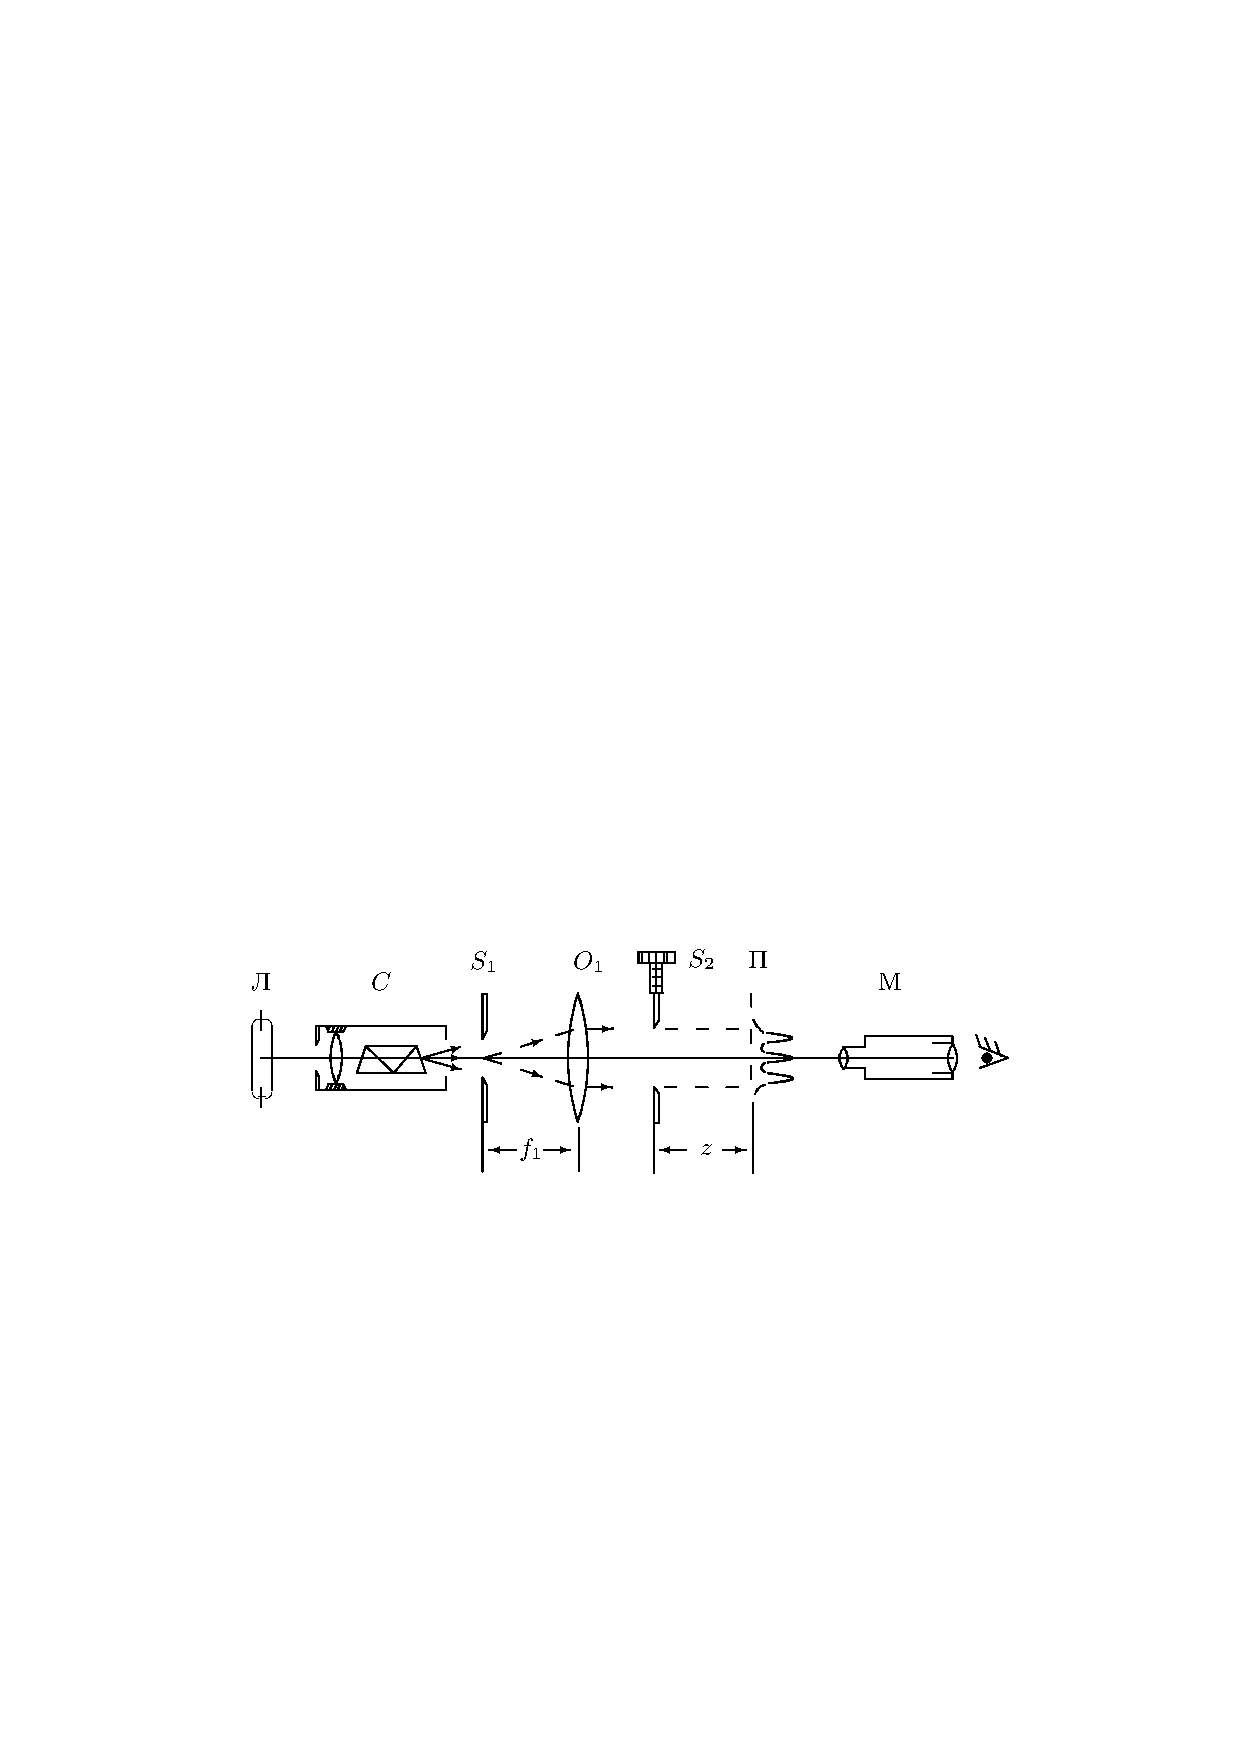
\includegraphics[width=0.8\linewidth]{a.pdf}
		\caption{Схема установки для наблюдения дифракции Френеля}
		\label{labA}
	\end{figure}
	
	Щель $ S_2 $ освещается параллельным пучком монохроматического света с помощью коллиматора, образованного объективом $ O_1 $, и щелью $S_1$, находящейся в его фокусе. На щель $ S_1 $ сфокусировано изображение спектральной линии, выделенной из спектра ртутной лампы Л при помощи простого монохроматора C, в котором используется призма прямого зрения. Распределение интенсивности света в плоскости наблюдения П проще всего рассчитывать с помощью зон Френеля (для щели их иногда называют зонами Шустера). При освещении щели $ S_2 $ параллельным пучком лучей (плоская волна) зоны Френеля представляют собой полоски, параллельные краям щели (рис. \ref{zone}). Результирующая амплитуда в точке наблюдения определяется суперпозицией колебаний от тех зон Френеля, которые не перекрыты створками щели. Графическое определение результирующей амплитуды производится с помощью векторной диаграммы --- спирали Корню. Суммарная ширина $ n $ зон Френеля (Шустера) определяется соотношением:
	
	\begin{equation}\label{xin}
		\xi_n = \sqrt{zn\lambda}
	\end{equation}
	где $ z $ --- расстояние от щели до плоскости наблюдения (рис. \ref{labA}), а $ \lambda $ --- длина волны.
	
	\begin{figure}[h!]
		\begin{center}
			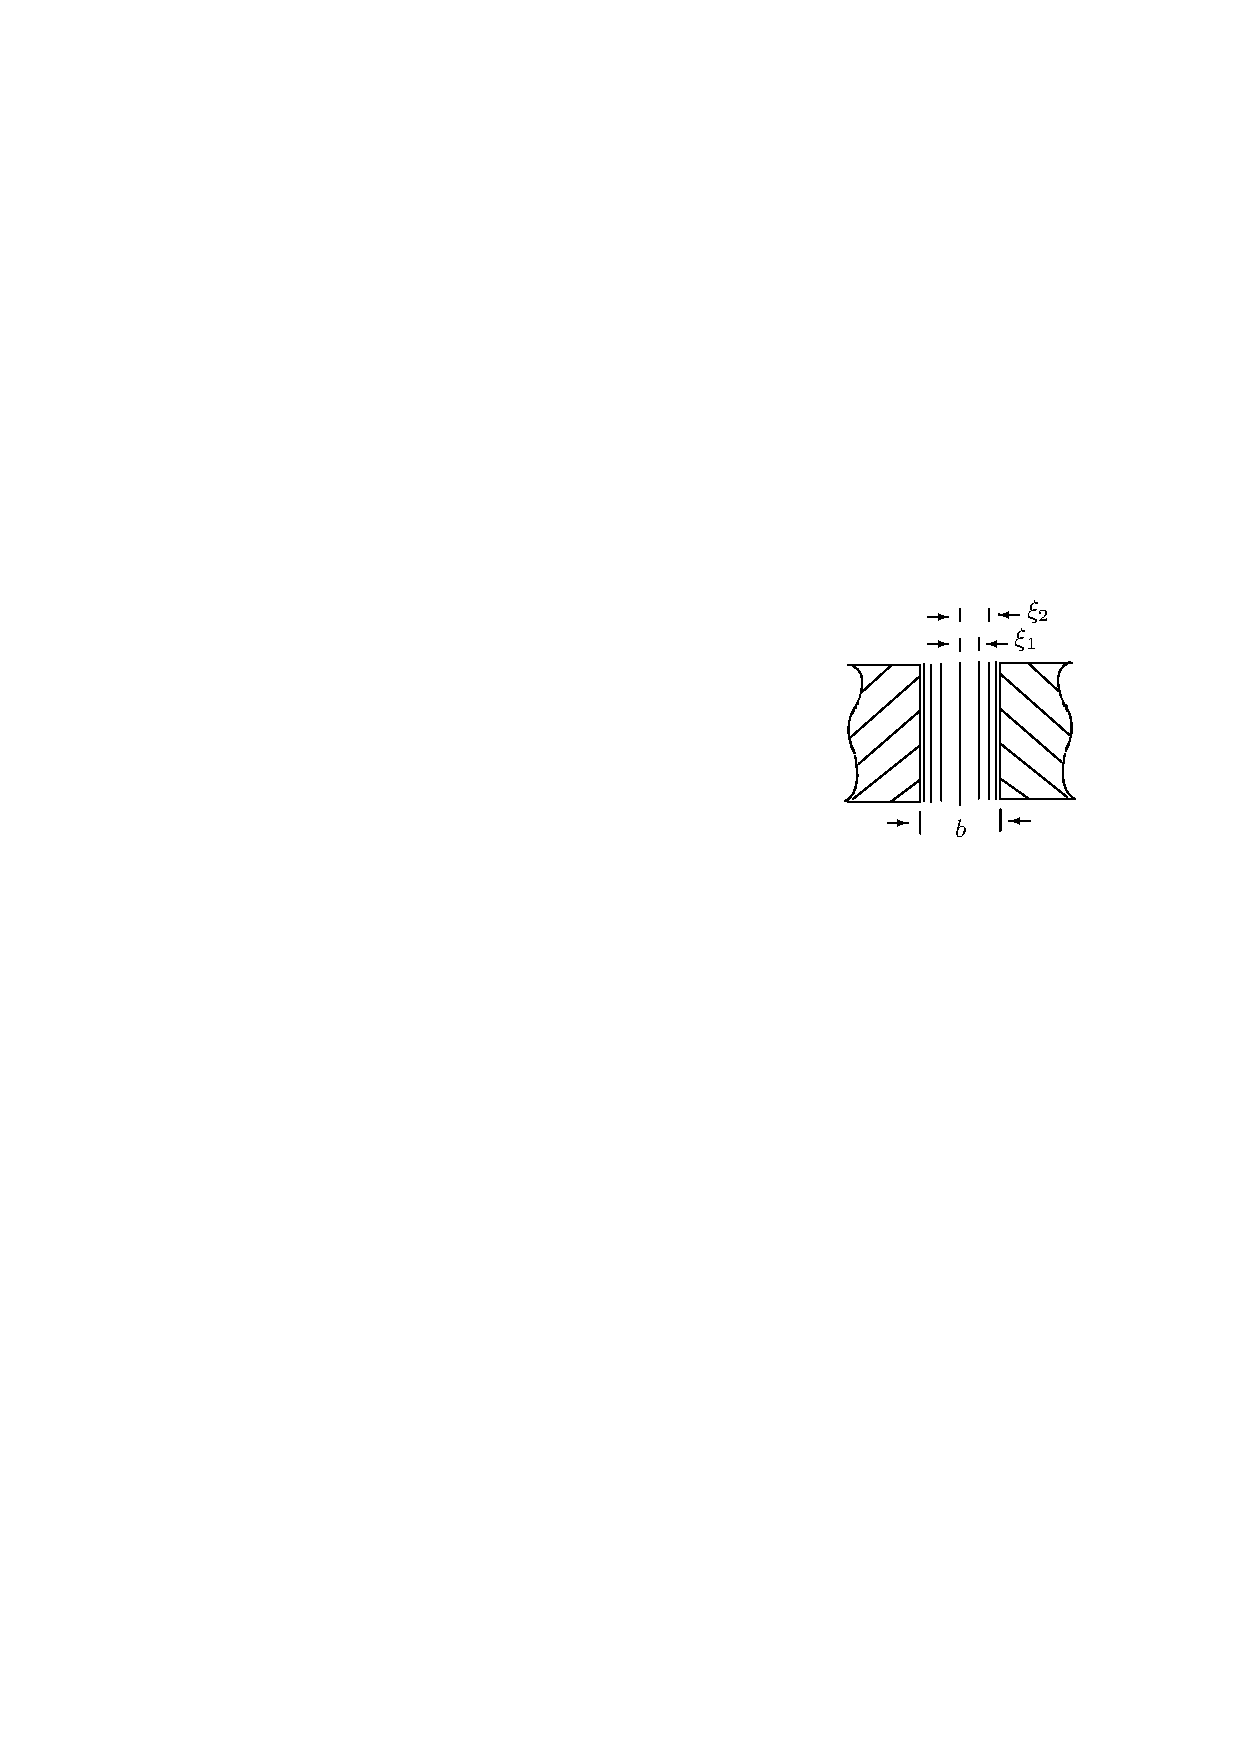
\includegraphics[width=0.3\linewidth]{zone}
		\end{center}
		\caption{Зоны Френеля}
		\label{zone}
	\end{figure}
	
	Вид наблюдаемой дифракционной картины
	на щели шириной $ b $ определяется волновым параметром $ p $ или числом Френеля $ C $ (число открытых полных зон):
	
	
	\begin{equation}\label{}
		p = \dfrac{\sqrt{z \lambda}}{b}, \qquad C = \dfrac{1}{p^2}
	\end{equation}
	
	Дифракционная картина отсутствует вблизи щели при $ p \ll 1 $ ($ C \gg 1 $, т. е. на щели укладывается огромное число зон), а распределение интенсивности света за щелью можно приближённо получить с помощью законов геометрической оптики. Дифракционная картина в этом случае наблюдается только в узкой области на границе света и тени у краёв экрана.
	
	При небольшом удалении от щели (или изменении ширины щели $ S_2 $) эти две группы дифракционных полос перемещаются практически независимо друг от друга. Каждая из этих групп образует картину дифракции Френеля на краю экрана. Распределение интенсивности при дифракции света на краю экрана может быть найдено с помощью спирали Корню.
	
	При дальнейшем увеличении расстояния $ z $ (или уменьшении ширины щели $ S_2 $) обе системы дифракционных полос постепенно сближаются и, наконец, при $ C \gtrsim 1 $ накладываются друг на друга. Распределение интенсивности в плоскости наблюдения в этом случае определяется числом зон Френеля, укладывающихся на полуширине щели $ b/2 $. Если это число равно $ n $, то в поле зрения наблюдается $ m = n - 1 $ тёмных полос. Таким образом, по виду дифракционной картины можно оценить число зон Френеля на полуширине щели.
	
	\subsubsection{Измерения и обработка результатов}
	
	Измерим первоначальную длину щели: $ b = (0.20 \pm 0.01)$ мм. Будем приближать микроскоп к щели, по мере этого снимем зависимость координаты микроскопа от числа $ n - 1 $ тёмных полос по формуле $ a_n = x_n - x_0 $, где $ x_0 = 548 $ мм --- положение нуля. Результаты занесём в таблицу. В таблицу также занесём результат вычисления величины $ 2\xi_n $ по формуле \eqref{xin}. При этом длина волны зелёного света $ \lambda = 5461 \cdot 10^{-10} $ м. 
	\begin{equation}
		\xi_n = \sqrt{zn\lambda}.
	\end{equation}
	
	
	\begin{table}[H]
		\centering
		\begin{tabular}{|c|c|c|c|c|}
			\hline
			$n$ & $x_n$, мм & $a_n$, мм & $\xi_n$, мм  & $\delta(\xi_n)$, мм \\ \hline
			1 & 537 & 11  & 0.25 & 0.02      \\ \hline
			2 & 540 & 8   & 0.30 & 0.02      \\ \hline
			3 & 542 & 6   & 0.31 & 0.02      \\ \hline
			4 & 544 & 4   & 0.30 & 0.02      \\ \hline
			5 & 544 & 4   & 0.33 & 0.02      \\ \hline
		\end{tabular}
	\caption{Зависимость темных полос от положения микроскопа}
	\end{table}
	По полученным данным построим график, проверим тот факт, что количество темных полос линейно зависит от расстояния на котором установлен микроскоп.
	\begin{figure}[H]
		\centering
		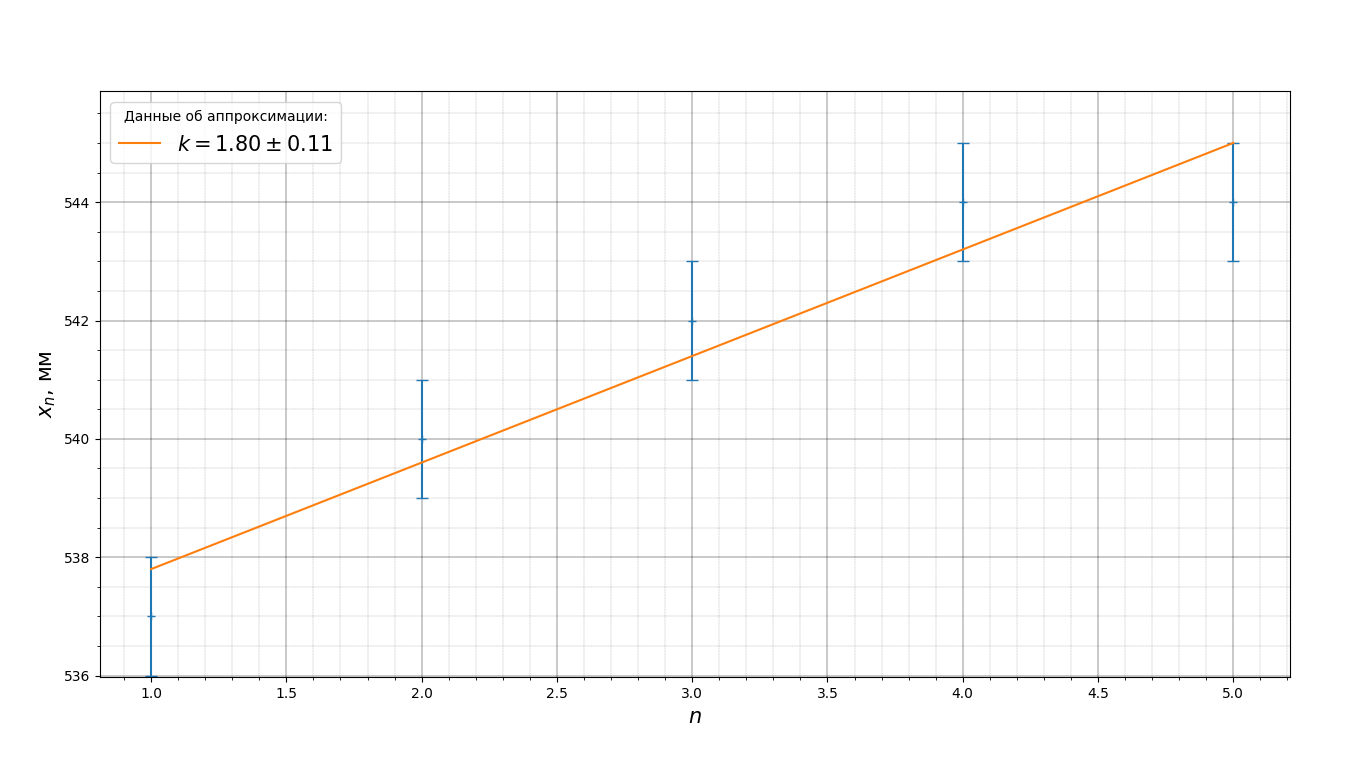
\includegraphics[width=0.9\linewidth]{Figure_1}
		\caption{Зависимость координаты микроскопа от числа темных полос}
		\label{fig:figure1}
	\end{figure}
	 Измерим размер щели $b$:\\
	 1) По делениям на окулярной шкале: $b = 0.44 \pm 0.04$ мм\\
	 2) По микрометрическому винту: $b = 0.37 \pm 0.01$ мм\\
	 
	 \subsection{Дифракция Фраунгофера на одной щели}
	 
	 \subsubsection{Экспериментальная установка}
	 
	 На значительном удалении от щели, когда выполнено условие $ C \ll 1 $
	 (то есть ширина щели становится значительно меньше ширины первой
	 зоны Френеля, $ b \ll \sqrt{\lambda z} $), изображение щели размывается и возникает
	 дифракционная картина, называемая дифракцией Фраунгофера.
	 
	 Дифракцию Френеля и Фраунгофера можно наблюдать на одной
	 и той же установке (рис. \ref{labA}). Однако при обычных размерах установки дифракция Фраунгофера возникает только при очень узких щелях.
	 
	 \begin{figure}[h!]
	 	\centering
	 	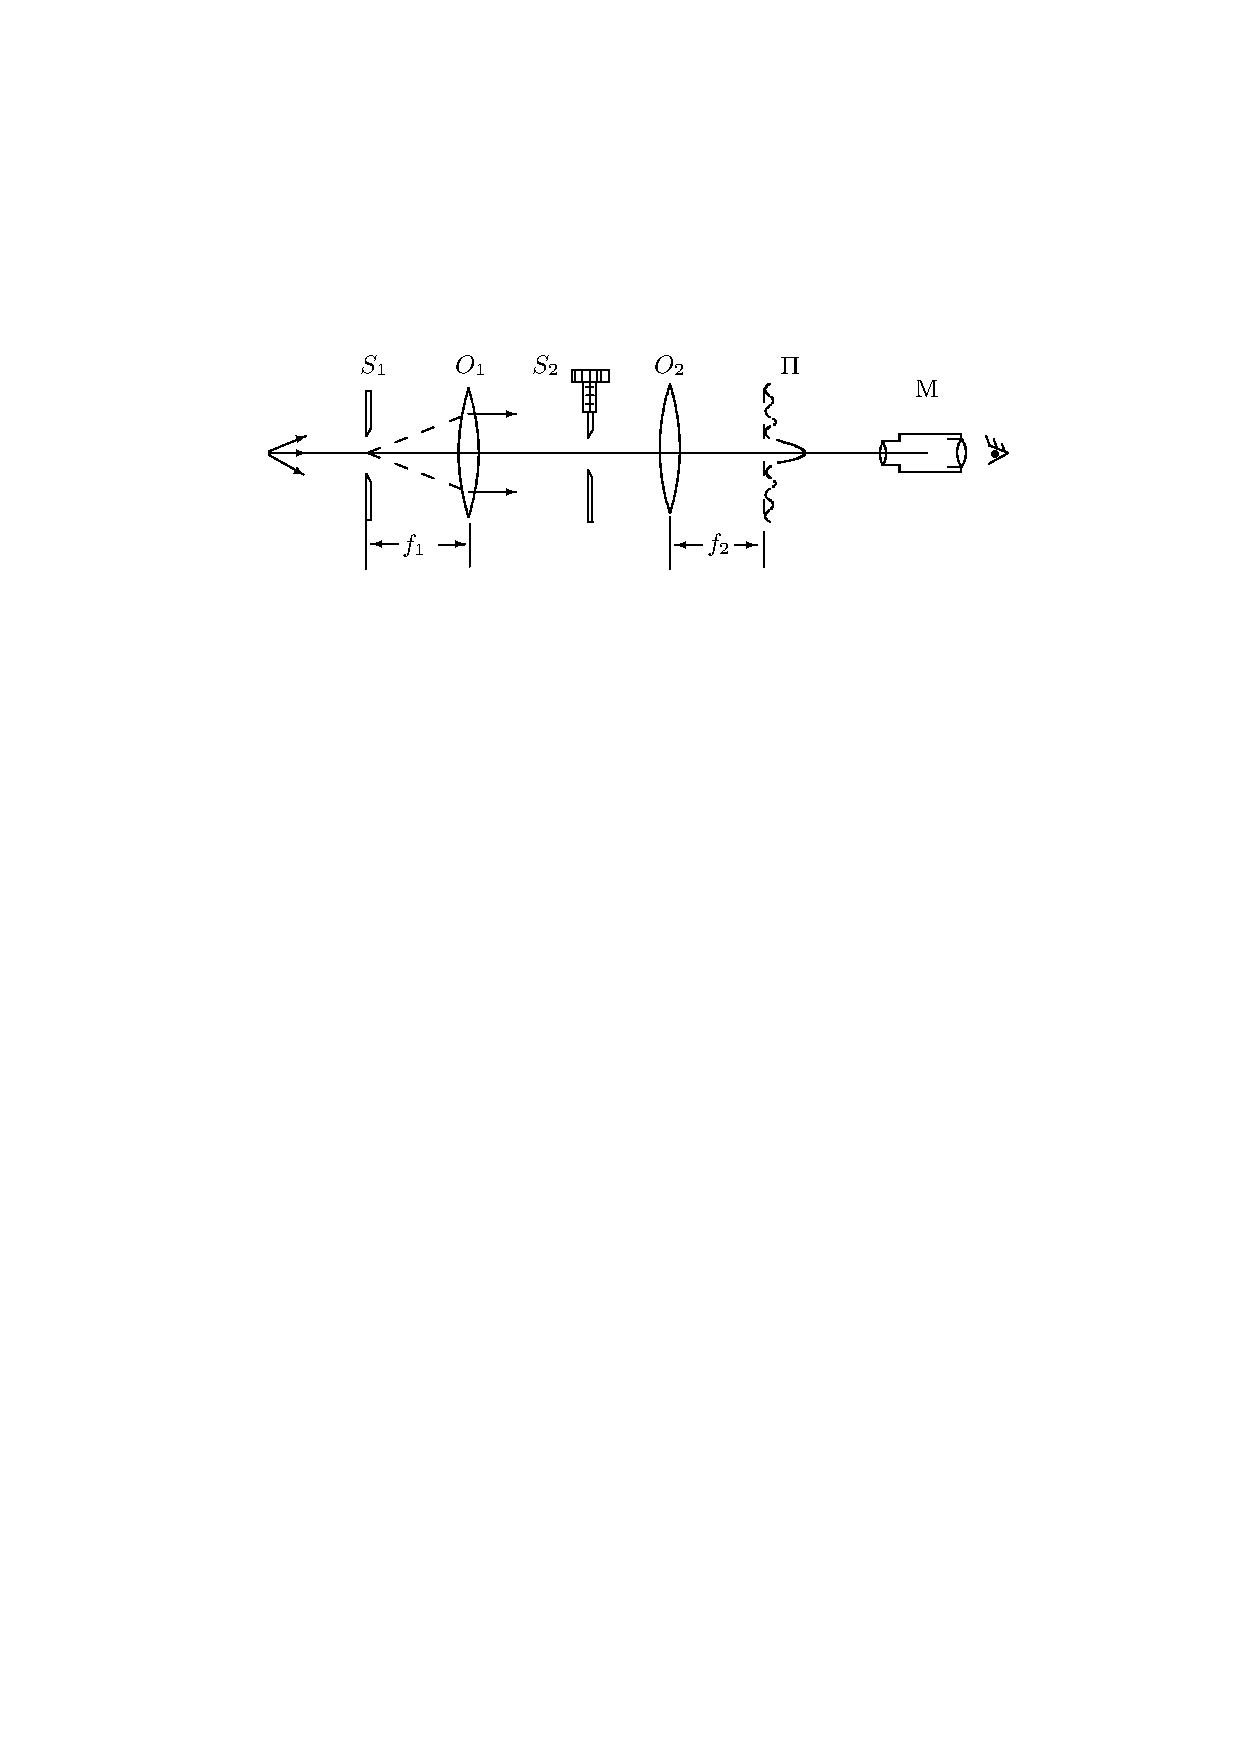
\includegraphics[width=0.8\linewidth]{b.pdf}
	 	\caption{Схема установки для наблюдения дифракции Фраунгофера на щели}
	 	\label{labB}
	 \end{figure}
	 
	 Например, при $ z \approx  20-40 $  см и $  \lambda \approx 5 \cdot 10^{-5}  $   см получаем $  b \ll 0,3 $ мм. Поскольку работать с такими тонкими щелями неудобно, для наблюдения дифракции Фраунгофера к схеме, изображённой на рис. \ref{labA}, добавляется объектив $ O_2  $ (рис. \ref{labB}).
	 
	 Дифракционная картина наблюдается здесь в фокальной плоскости
	 объектива $ O_2 $. Каждому значению угла $ \theta $ соответствует в этой плоскости точка, отстоящая от оптической оси на расстоянии
	 
	 \begin{equation}\label{x}
	 	x = f_2 \tg \theta \approx f_2 \theta
	 \end{equation}
	 
	 Поскольку объектив не вносит дополнительной разности хода
	 между интерферирующими лучами (таутохронизм), в его фокальной
	 плоскости наблюдается неискаженная дифракционная картина Фраунгофера. Эта картина соответствует бесконечно удалённой плоскости
	 наблюдения.
	 
	 В центре поля зрения наблюдается дифракционный максимум (светлая полоса). При малых углах $ \theta $ положение минимумов (тёмных полос)
	 определяется, соотношением
	 
	 \begin{equation}\label{theta_m}
	 	\theta_m = m \dfrac{\lambda}{b}
	 \end{equation}
	 
	 Расстояние $ x_m $ от тёмной полосы до оптической оси объектива $ O_2 $ пропорционально фокусному расстоянию $ f_2 $. Из \eqref{x} и \eqref{theta_m} следует 
	 
	 \begin{equation}\label{xm}
	 	x_m = m \dfrac{\lambda}{b} f_2
	 \end{equation}
	 
	 Видно, что при малых углах минимумы эквидистантны, а расстояния $ \delta x $ между минимумами обратно пропорциональны ширине $ b $ щели $ S_2 $.
	 
	 \subsubsection{Измерения и обработка результатов}
	 ПО микрометрической шкале измерим ширину щели и получим: $b = (0.28 \pm 0.01)$ мм, фокусное расстояние линзы $f_2 = 12.5$ см.
	 Снимем зависимость координаты некоторых минимумов, приведем данные в таблицу и построим график.
	 \begin{table}[H]
	 	\centering
	 	\begin{tabular}{|c|c|c|c|c|c|c|c|c|c|c|}
	 		\hline
	 		$n$   & -5 & -4 & -3 & -2 & -1 & 1  & 2  & 3  & 4  & 5  \\ \hline
	 		$x_n$, дел & 60 & 50 & 40 & 30 & 20 & 15 & 25 & 35 & 45 & 55 \\ \hline
	 	\end{tabular}
 	\caption{расстояния до некоторых минимумов}
	 \end{table}
 	Построим теперь график зависимости переведя расстояние в абсолютные координаты.
 	\begin{figure}[H]
 		\centering
 		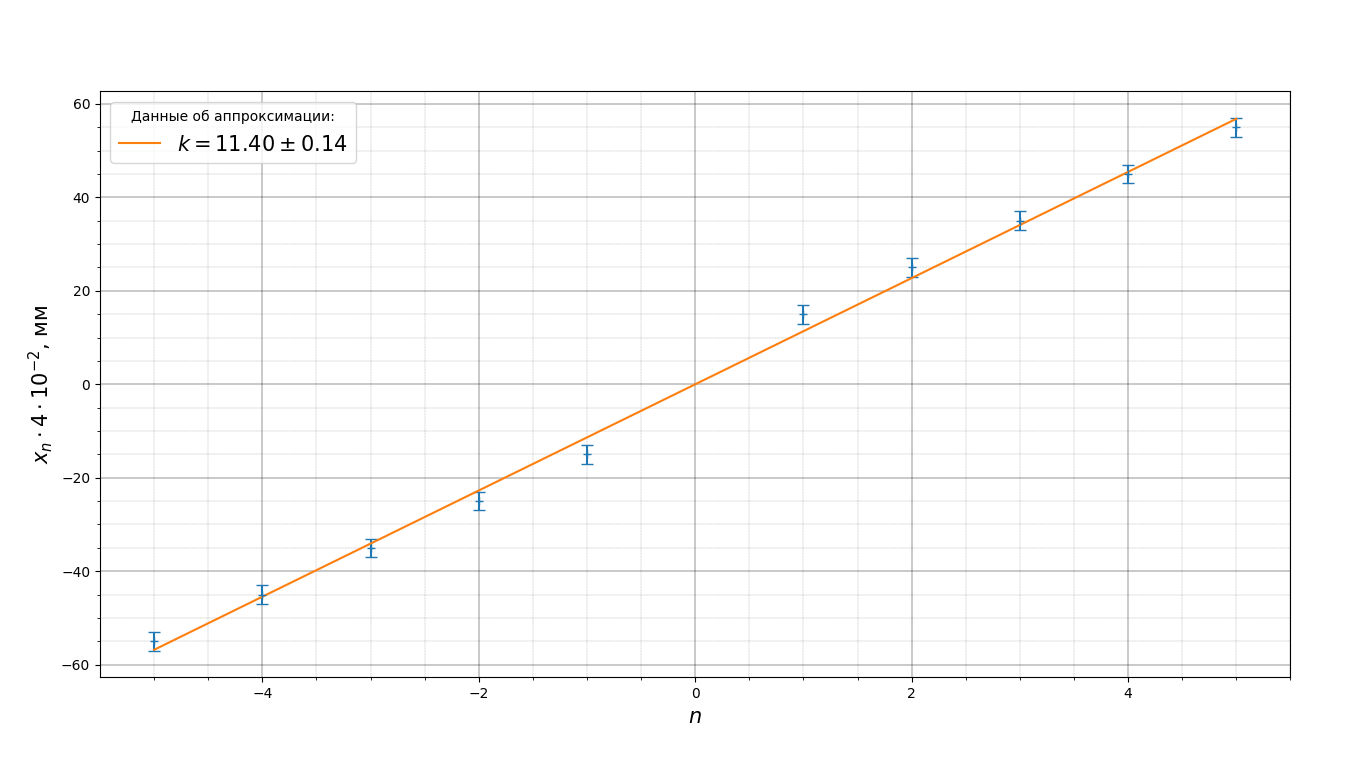
\includegraphics[width=0.9\linewidth]{Figure_2}
 		\caption{Зависимость координаты минимума от его номера}
 		\label{fig:figure2}
 	\end{figure}
 	Переводя в миллиметры получим угол наклона равный: $k = (22.8 \pm 0.3)\cdot 10^{-2}$ мм.
 	ПО формуле 6 найдем размер щели: $b = \frac{\lambda}{k}f_2 = (30.1 \pm 4.1) \cdot 10^{-2}$ мм.
 	\subsection{Дифракция Фраунгофера на двух щелях}
 	
 	\subsubsection{Экспериментальная установка}
 	
 	Для наблюдения дифракции Фраунгофера на двух щелях в установке (рис. \ref{labB}) следует заменить щель $ S_2 $ экраном Э с двумя щелями
 	(рис. \ref{labC}). При этом для оценки влияния ширины входной щели на чёткость дифракционной картины вместо входной щели $ S_1 $ следует поставить щель с микрометрическим винтом. Два дифракционных изображения входной щели, одно из которых образовано лучами, прошедшими через левую, а другое --- через правую щели, накладываются друг на друга.
 	
 	\begin{figure}[h!]
 		\centering
 		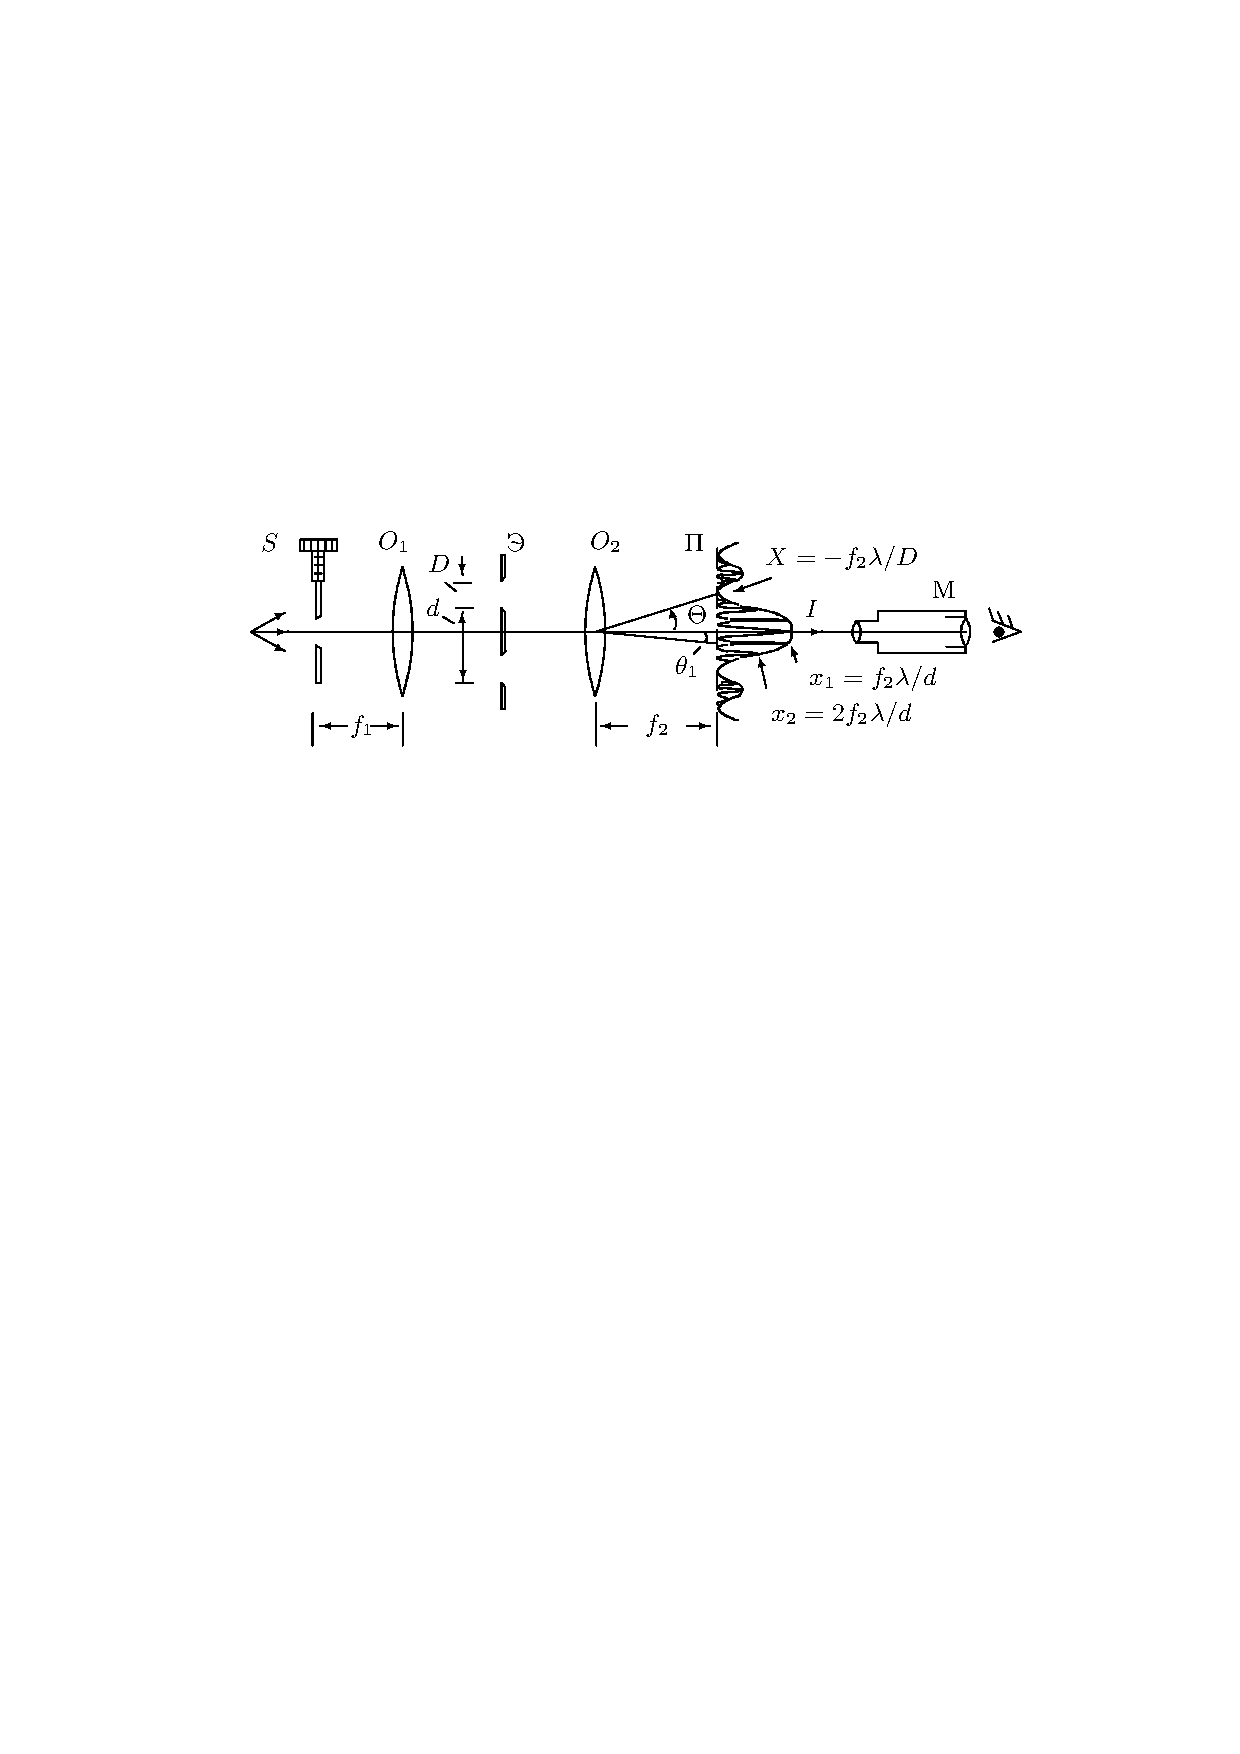
\includegraphics[width=0.8\linewidth]{c.pdf}
 		\caption{Схема установки для наблюдения дифракции Фраунгофера на двух щелях}
 		\label{labC}
 	\end{figure}
 	
 	Если входная щель достаточно узка, то дифракционная картина
 	в плоскости П (рис. \ref{labC}) подобна той, что получалась при дифракции
 	на одной щели (рис. \ref{labB}), однако теперь вся картина испещрена рядом
 	дополнительных узких полос.
 	Угловая координата $ \theta_m $ интерференционного максимума $ m $-го порядка определяется соотношением
 	
 	\begin{equation}\label{}
 		\theta_m = m \dfrac{\lambda}{b}
 	\end{equation}
 	
 	где $ d $ --- расстояние между щелями. Линейное расстояние $ \delta x $ между соседними интерференционными полосами в плоскости П равно, поэтому
 	
 	\begin{equation}\label{dx}
 		\delta x = f_2 \dfrac{\lambda}{d}
 	\end{equation}
 	
 	На рис. \ref{labC} показано распределение интенсивности в фокальной плоскости объектива $ O_2 $. Штриховой линией (в увеличенном масштабе)
 	изображено распределение интенсивности при дифракции света на одиночной щели. Нетрудно оценить число n интерференционных полос,
 	укладывающихся в области центрального дифракционного максимума.
 	Согласно \eqref{xm} полная ширина главного максимума равна $ 2 f_2 \lambda /b $, где $ b $ ширина щели, отсюда
 	
 	\begin{equation}\label{n}
 		n = \dfrac{2f_2 \lambda}{b} \dfrac{1}{\delta x} = \dfrac{2d}{b}
 	\end{equation}
 	
 	При дифракции света на двух щелях чёткая система интерференционных полос наблюдается только при достаточно узкой ширине входной щели $ S $, которую можно рассматривать как протяжённый источник света размером $ b $. Для наблюдения интерференции необходимо, чтобы расстояние $ d $между щелями не превышало радиуса когерентности
 	
 	\begin{equation}\label{}
 		d \ll \dfrac{\lambda}{b} f_1
 	\end{equation}
 	
 	Здесь $ b $ --- ширина входной щели $ S $ и, следовательно, $  b/f_1 $ --- её угловая ширина. Таким образом, по размытию интерференционной картины можно оценить размер источника. Этот метод используется в звёздном интерферометре при измерении угловых размеров звёзд.
 	
 	\subsubsection{Измерения и обработка результатов}
 	
 	\begin{figure}[H]
 		\centering
 		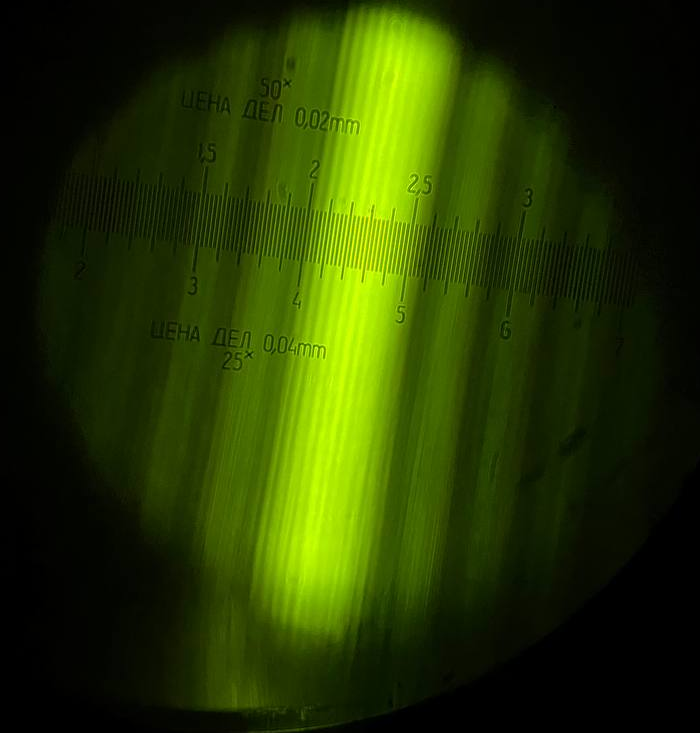
\includegraphics[width=0.6\linewidth]{screenshot001}
 		\caption{фото интерференционной картины}
 		\label{fig:screenshot001}
 	\end{figure}
 	
 	Получим на экране интересующую нас картинку, измерим количество полос и размеры щели.\\
 	Измерили: $n = 9$, $L = 0.72\pm 0.04$ мм.
 	Рассчитаем:\\ $\delta x = L / n = 0.08$ мм - расстояние между соседними полосами, \\$d = f_2 \lambda / \delta x = 0.85 \pm 0.02$ мм - расстояние между щелями, \\$b = 2d / n = 0.19\pm 0.01$ мм - ширина щели.\\
 	Также при помощи микроскопа измерим параметры щелей $ d $ и $ b $ прямо. Получаем\\
 	$d_\text{микр} = (0.96 \pm 0.02) \text{ мм}, $\\
 	$b_\text{микр} = (0.22 \pm 0.02) \text{ мм}.$\\
 	\subsection{Влияние дифракции на разрешающую способность оптического инструмента}
 	
 	\subsubsection{Экспериментальная установка}
 	
 	Установка, представленная на рис. \ref{labB}, позволяет исследовать влияние дифракции на разрешающую способность оптических инструментов.
 	
 	Как уже было выяснено, линзы $O_1$ и $ O_2$ в отсутствие щели $S_2$ создают в плоскости П изображение щели $S_1$, и это изображение рассматривается в микроскоп М. Таким образом, нашу установку можно рассматривать как оптический инструмент, предназначенный для получения изображения предмета. При этом коллиматор (щель $S_1$ и объектив $O_1$) является моделью далёкого предмета, а объектив $O_2$ и микроскоп М составляют зрительную трубу, наведённую на этот предмет.
 	Щель $S_2$, установленная непосредственно перед объективом $O_2$, позволяет изменять эффективный размер объектива и, следовательно, разрешающую способность оптической системы.
 	
 	\begin{figure}[h!]
 		\centering
 		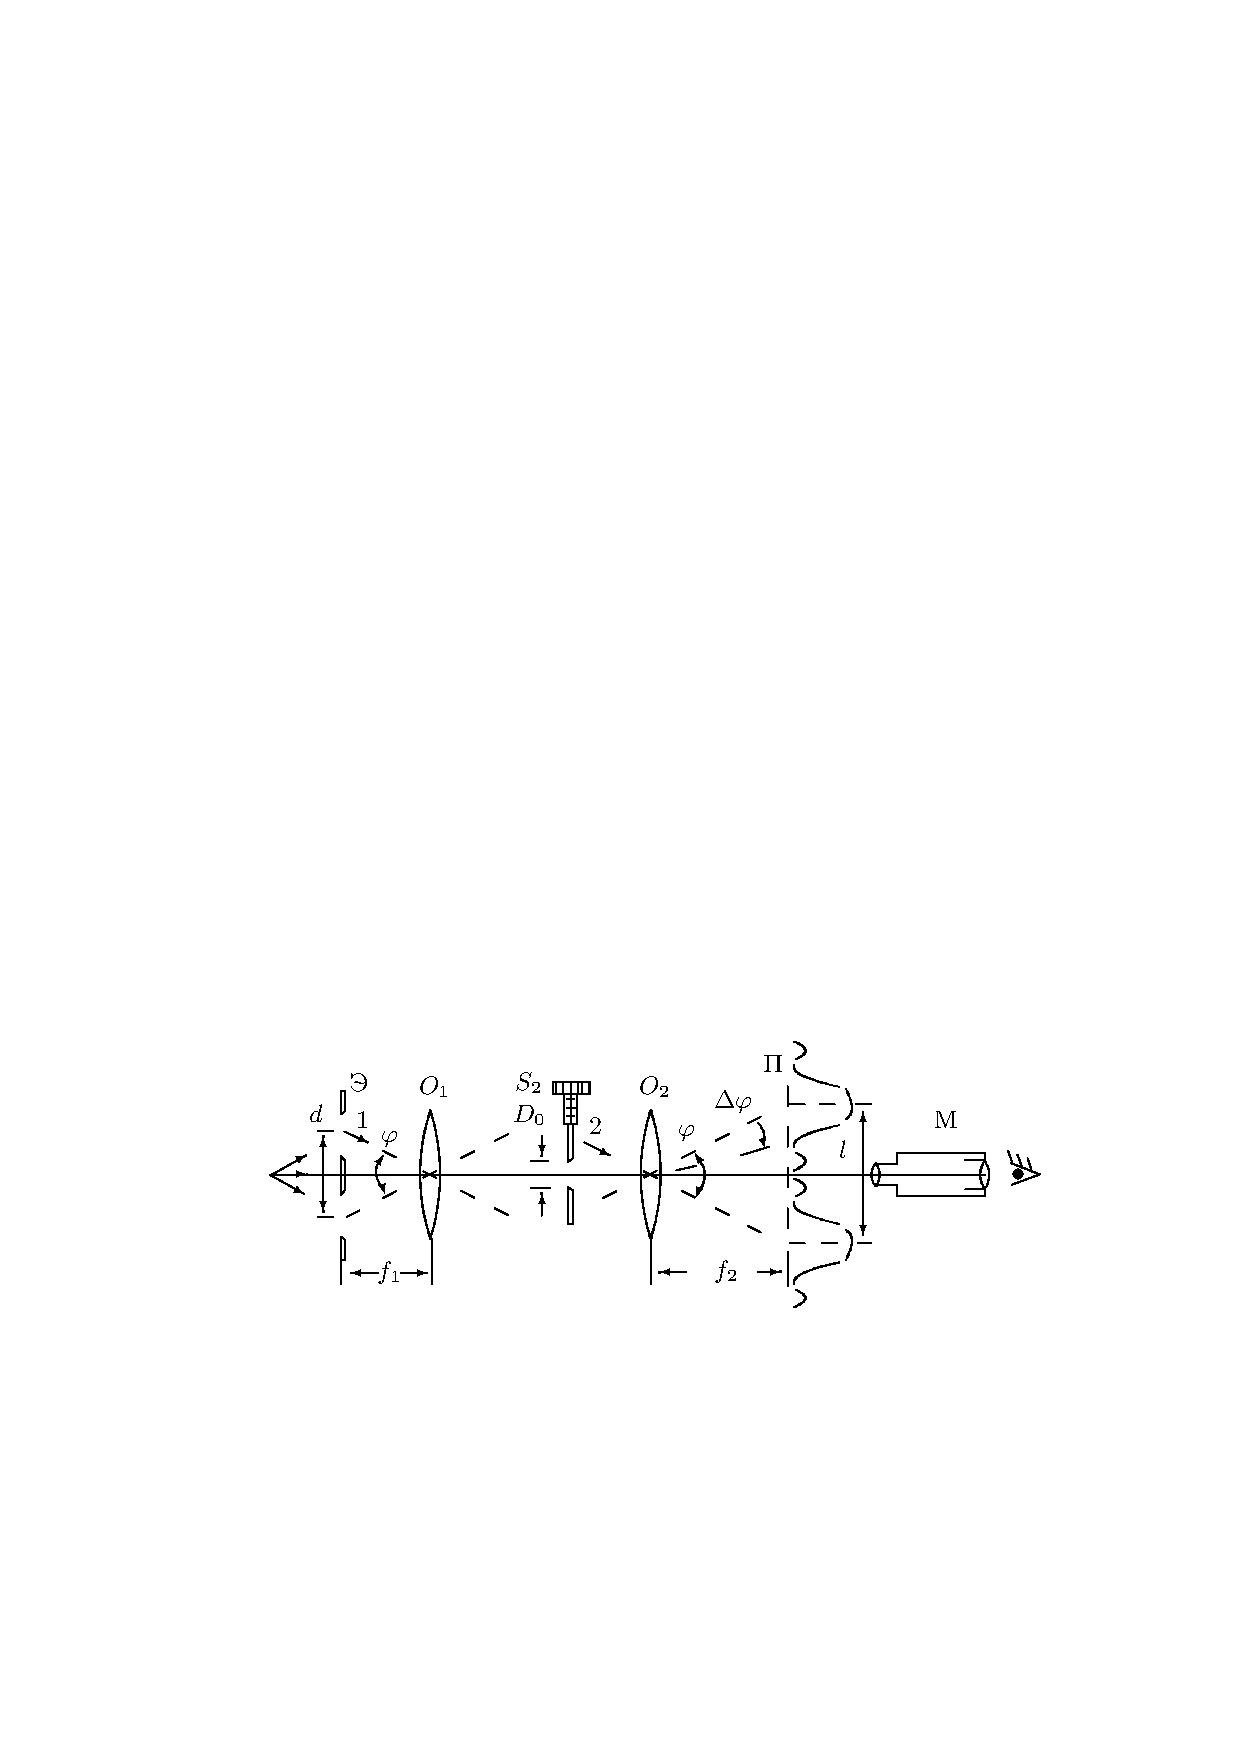
\includegraphics[width=0.8\linewidth]{d.pdf}
 		\caption{Схема установки для исследования разрешающей
 			способности оптического инструмента}
 		\label{labG}
 	\end{figure}
 	
 	Поместим вместо щели $S_1$ экран Э с двумя узкими щелями, расстояние между которыми равно $d$ (рис. \ref{labG}). Тогда расстояние $l$ между изображениями щелей в плоскости П равно
 	\begin{equation}
 		l = \varphi f_2 = d \dfrac{f_2}{f_1},
 	\end{equation}
 	а ширина каждого изображения
 	\begin{equation}
 		\delta x \approx \dfrac{\lambda}{b} f_2
 	\end{equation}
 	определяется дифракцией света на щели $S_2$. Когда полуширина дифракционного изображения превышает расстояние между изображениями, то по виду дифракционной картины трудно определить, представляет собой источник двойную или одиночную щель.
 	
 	Условия, при которых ещё можно различить, имеем мы дело с одной или двумя щелями, для разных наблюдателей различны. Для того чтобы исключить связанный с этим произвол, пользуются обычно критерием Рэлея, который приблизительно соответствует возможностям визуального наблюдения: изображения считаются различимыми, когда максимум одного дифракционного пятна совпадает с минимумом другого, а в условиях нашей задачи --- когда полуширина дифракционного изображения $\delta x$ совпадает с расстоянием $l$ между изображениями отдельных щелей:
 	\begin{equation}
 		\delta x \sim l \to \dfrac{\lambda}{b} \sim \dfrac{d}{f_1}.
 	\end{equation}
 	
 	\subsubsection{Измерения и обработка результатов}
 	
 	Для проверки справедливости критерия Рэлея сравним измеренную ширину $b_0$ щели $S_2$, при которой изображение двух щелей сливается, но всё ещё различимо, с расчётом по формуле $\lambda f_1/d$.
 	
 	\begin{table}[h!]
 		\centering
 		\caption{Измерения}
 		\begin{tabular}{|c|c|} \hline
 			$b_0$, $10^{-2}$ мм &	$\lambda f_1/d$, $10^{-2}$ мм \\
 			\hline
 			27.4 &	6.0 \\ \hline
 		\end{tabular}   
 	\end{table}
 	\section{Выводы}
 	Изучили два типа дифракции: Френеля и Фраунгофера; в случае Фраунгофера изучили явление дифракции на одной и двух щелях.\\
 	
 	\textbf{Дифракция Френеля.} По результатам измерений и проведённых вычислений можно утверждать, что полученная ширина щели примерно одинакова в случае прямого вычисления и в случаем вычисления при помощи замеров координат минимумов.
 	
 	Кроме того, при дифракции на препятствии при удалении микроскопа от нити на её фоне всегда наблюдали чётное число тёмных дифракционных полос и светлый центр.
 	
 	\textbf{Дифракция Фраунгофера на одной щели.} Значение для ширины щели
 	\begin{equation*}
 		b_\text{экс} =  (30.1 \pm 4.1) \cdot 10^{-2} \; \text{мм} 
 	\end{equation*}
 	вычисленное по формуле, совпадает в пределах погрешности с величиной, измеренной по микрометрической шкалой:
 	\begin{equation*}
 		b_\text{мкм} =  (28.0 \pm 1.0) \cdot 10^{-2} \; \text{мм}.
 	\end{equation*}
 	Это подтверждает теоретические выкладки и говорит о выполнении предложенной теории.\\
 	
 	\textbf{Дифракция Фраунгофера на двух щелях.} Измеренные экспериментально ширина щели и расстояние между щелями совпадают с измеренными напрямую.\\
 	$d_\text{экс} = (0.85 \pm 0.02) \text{ мм},$\\
 	$b_\text{экс} = (0.19 \pm 0.01) \text{ мм},$\\
 	$d_\text{мкм} = (0.96 \pm 0.02) \text{ мм}, \varepsilon = 11 \%,$\\
 	$b_\text{мкм} = (0.22 \pm 0.02) \text{ мм}, \varepsilon = 13.6 \%.$\\
 	
 	\textbf{Влияние дифракции на разрешающую способность оптического инструмента}. В результате измерений получаем, что $b_0 > \lambda f_1/d$, что означает разрешимость изображений по Рэлею, что мы и наблюдали в ходе выполнения работы.
 	
 	
 	

\end{document}